\documentclass[11pt,a4paper]{article}
\usepackage[margin=0.75in]{geometry}
\usepackage{amsmath,amssymb}
\usepackage{tikz}
\usepackage{enumitem}
\usepackage{xcolor}
\usepackage{tcolorbox}
\usepackage{fancyhdr}

\usetikzlibrary{shapes,arrows,positioning,fit,backgrounds}

\pagestyle{fancy}
\fancyhf{}
\rhead{Sampling Techniques Viva Guide}
\lhead{\thepage}

\definecolor{defcolor}{RGB}{230,240,255}
\definecolor{keycolor}{RGB}{255,240,230}

\title{\textbf{Sampling Techniques: Comprehensive Viva Guide}}
\author{Quick Reference for Oral Examination}
\date{}

\begin{document}
\maketitle

\section{Definitions and Core Concepts}

\begin{tcolorbox}[colback=defcolor,colframe=blue!50!black,title=\textbf{Random Sampling}]
\textbf{Definition:} A sampling method where each element in the population has an \emph{equal and independent} probability of being selected.

\textbf{Key Properties:}
\begin{itemize}[leftmargin=*,itemsep=0pt]
    \item Probability of selection: $P(x_i) = \frac{1}{N}$ for population size $N$
    \item Each selection is independent of others
    \item Simple Random Sampling (SRS) is the foundation of statistical inference
\end{itemize}
\end{tcolorbox}

\begin{tcolorbox}[colback=defcolor,colframe=blue!50!black,title=\textbf{Stratified Sampling}]
\textbf{Definition:} The population is divided into homogeneous subgroups (strata) based on a characteristic, and random samples are drawn from each stratum.

\textbf{Key Properties:}
\begin{itemize}[leftmargin=*,itemsep=0pt]
    \item Population = $\bigcup_{h=1}^{L} S_h$ where $S_h$ are disjoint strata
    \item Sample from each stratum: $n_h$ from stratum $h$
    \item Total sample size: $n = \sum_{h=1}^{L} n_h$
    \item Ensures representation from all subgroups
\end{itemize}
\end{tcolorbox}

\begin{tcolorbox}[colback=keycolor,colframe=red!50!black,title=\textbf{Hybrid Sampling (CRITICAL)}]
\textbf{Definition:} A two-stage approach combining stratified sampling with random sampling within strata. First stratify, then apply different sampling rates or methods per stratum.

\textbf{Key Characteristics:}
\begin{itemize}[leftmargin=*,itemsep=0pt]
    \item Combines advantages of both stratification and random sampling
    \item Allocation can be proportional or optimal
    \item Reduces variance compared to simple random sampling
    \item Flexible: can oversample rare strata
\end{itemize}
\end{tcolorbox}

\begin{tcolorbox}[colback=defcolor,colframe=blue!50!black,title=\textbf{Stratified Clustering}]
\textbf{Definition:} A multi-stage technique where the population is first divided into strata, then clusters are formed within strata, and samples are drawn from selected clusters.

\textbf{Structure:}
\begin{itemize}[leftmargin=*,itemsep=0pt]
    \item Stage 1: Divide population into strata
    \item Stage 2: Identify clusters within each stratum
    \item Stage 3: Sample clusters, then sample elements within clusters
    \item Useful for geographically dispersed populations
\end{itemize}
\end{tcolorbox}

\section{Mathematical Foundations}

\subsection{Random Sampling}
\textbf{Sample Mean Estimator:}
$$\bar{x} = \frac{1}{n}\sum_{i=1}^{n} x_i$$

\textbf{Variance of Sample Mean:}
$$\text{Var}(\bar{x}) = \frac{\sigma^2}{n}\left(1-\frac{n}{N}\right) = \frac{\sigma^2}{n} \cdot \text{FPC}$$
where FPC = finite population correction = $(1-\frac{n}{N})$

\textbf{Standard Error:}
$$SE(\bar{x}) = \sqrt{\frac{s^2}{n}\left(1-\frac{n}{N}\right)}$$

\subsection{Stratified Sampling}
\textbf{Stratified Mean Estimator:}
$$\bar{x}_{st} = \sum_{h=1}^{L} W_h \bar{x}_h$$
where $W_h = \frac{N_h}{N}$ is the weight of stratum $h$, and $\bar{x}_h$ is the sample mean in stratum $h$.

\textbf{Variance of Stratified Mean:}
$$\text{Var}(\bar{x}_{st}) = \sum_{h=1}^{L} W_h^2 \frac{\sigma_h^2}{n_h}\left(1-\frac{n_h}{N_h}\right)$$

\textbf{Allocation Methods:}
\begin{itemize}[itemsep=0pt]
    \item \textit{Proportional:} $n_h = n \cdot W_h = n \cdot \frac{N_h}{N}$
    \item \textit{Optimal (Neyman):} $n_h = n \cdot \frac{N_h\sigma_h}{\sum_{k=1}^{L}N_k\sigma_k}$
    \item Optimal allocation minimizes variance for fixed cost
\end{itemize}

\subsection{Hybrid Sampling}
Hybrid sampling variance depends on the specific combination used. For stratified random sampling hybrid:
$$\text{Var}(\bar{x}_{hybrid}) \leq \text{Var}(\bar{x}_{SRS})$$

The reduction factor depends on stratum homogeneity and allocation efficiency.

\section{Practical Understanding}

\subsection{When to Use Each Technique}

\begin{center}
\begin{tabular}{|p{3cm}|p{4.5cm}|p{5cm}|}
\hline
\textbf{Technique} & \textbf{Best Used When} & \textbf{Example} \\
\hline
Random Sampling & Homogeneous population, no prior knowledge & Selecting students from a single class \\
\hline
Stratified & Known heterogeneous subgroups, want precision & Income survey across age groups \\
\hline
Hybrid & Need flexibility, multiple characteristics & Customer satisfaction with regional and age stratification \\
\hline
Stratified Clustering & Large geographic area, cost constraints & National health survey by state then city \\
\hline
\end{tabular}
\end{center}

\subsection{Decision Flowchart}

\begin{center}
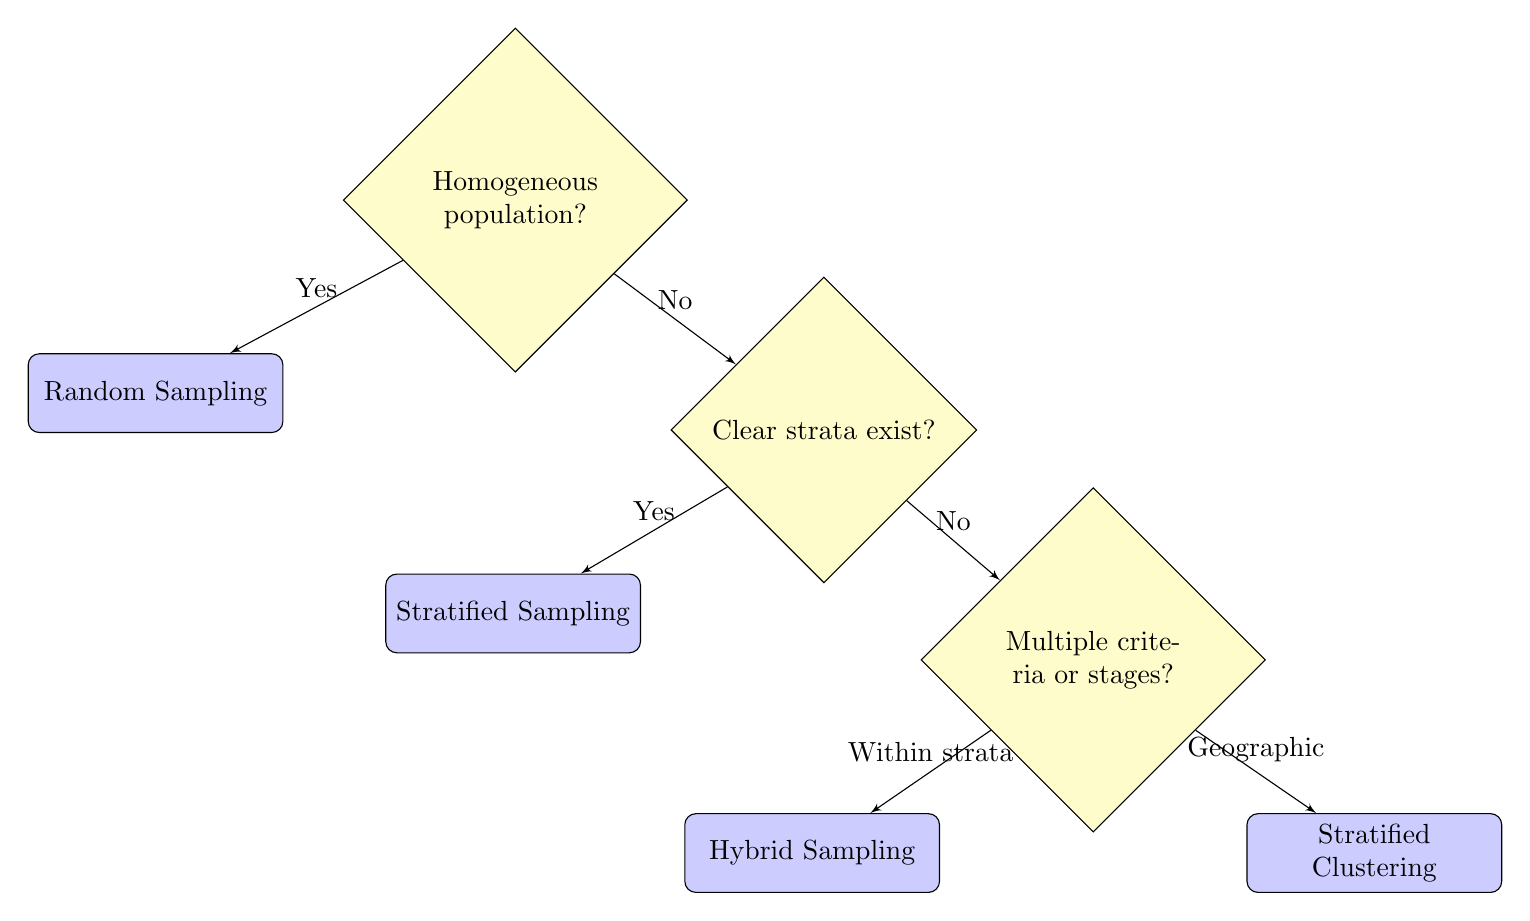
\begin{tikzpicture}[
    node distance=1.2cm,
    decision/.style={diamond, draw, fill=yellow!20, text width=3.5cm, text centered, inner sep=1pt},
    block/.style={rectangle, draw, fill=blue!20, text width=3cm, text centered, rounded corners, minimum height=1cm},
    line/.style={draw, -latex'}
]

\node [decision] (start) {Homogeneous population?};
\node [block, below left=of start, xshift=-1cm] (random) {Random Sampling};
\node [decision, below right=of start, xshift=1cm] (strata) {Clear strata exist?};
\node [block, below left=of strata, xshift=-0.5cm] (stratified) {Stratified Sampling};
\node [decision, below right=of strata, xshift=0.5cm] (multi) {Multiple criteria or stages?};
\node [block, below left=of multi] (hybrid) {Hybrid Sampling};
\node [block, below right=of multi] (cluster) {Stratified Clustering};

\path [line] (start) -- node [above] {Yes} (random);
\path [line] (start) -- node [above] {No} (strata);
\path [line] (strata) -- node [above] {Yes} (stratified);
\path [line] (strata) -- node [above] {No} (multi);
\path [line] (multi) -- node [above] {Within strata} (hybrid);
\path [line] (multi) -- node [above] {Geographic} (cluster);

\end{tikzpicture}
\end{center}

\section{Common Viva Questions with Detailed Answers}

\subsection*{Q1: What is the main advantage of stratified sampling over random sampling?}
\textbf{Answer:} Stratified sampling provides \emph{greater precision} (lower variance) than simple random sampling for the same sample size. This occurs because:
\begin{itemize}[itemsep=0pt]
    \item Within-stratum variance is smaller than population variance
    \item We ensure representation from all subgroups
    \item Mathematical proof: $\text{Var}(\bar{x}_{st}) \leq \text{Var}(\bar{x}_{SRS})$ when strata are homogeneous
    \item The gain is maximum when strata are internally homogeneous but differ from each other
\end{itemize}

\subsection*{Q2: Explain hybrid sampling and why it's useful.}
\textbf{Answer:} Hybrid sampling combines multiple sampling techniques, typically stratified sampling followed by different methods within strata. 

\textbf{Key benefits:}
\begin{itemize}[itemsep=0pt]
    \item \textit{Flexibility:} Can use different sampling rates for different strata
    \item \textit{Efficiency:} Oversample rare but important subgroups
    \item \textit{Cost-effective:} Apply expensive methods only where needed
    \item \textit{Precision:} Maintains stratification benefits while adapting to constraints
\end{itemize}

\textbf{Example:} In a national survey, stratify by region, then use cluster sampling in rural areas (cost-effective) and simple random sampling in urban areas (more precise).

\subsection*{Q3: How does stratified clustering differ from stratified sampling?}
\textbf{Answer:} 
\begin{itemize}[itemsep=0pt]
    \item \textbf{Stratified Sampling:} Sample individuals directly from each stratum
    \item \textbf{Stratified Clustering:} Sample clusters from each stratum, then sample individuals from selected clusters
\end{itemize}

\textbf{Key differences:}
\begin{enumerate}[itemsep=0pt]
    \item \textit{Stages:} Stratified clustering is multi-stage; stratified sampling is single-stage
    \item \textit{Sampling unit:} Clusters first, then individuals vs. individuals directly
    \item \textit{Cost:} Clustering reduces travel/administrative costs
    \item \textit{Variance:} Clustering typically increases variance due to intra-cluster correlation
\end{enumerate}

\subsection*{Q4: What is the finite population correction (FPC) and when is it important?}
\textbf{Answer:} FPC = $(1-\frac{n}{N})$ accounts for sampling without replacement from finite populations.

\textbf{When important:}
\begin{itemize}[itemsep=0pt]
    \item When sampling fraction $\frac{n}{N} > 0.05$ (5\% rule)
    \item Reduces estimated variance
    \item As $n \to N$, variance $\to 0$ (census)
    \item Often ignored for large populations where $\frac{n}{N} \approx 0$
\end{itemize}

\subsection*{Q5: Derive or explain the stratified mean estimator.}
\textbf{Answer:} The stratified mean is a weighted average of stratum means:
$$\bar{x}_{st} = \sum_{h=1}^{L} W_h \bar{x}_h$$

\textbf{Intuition:}
\begin{itemize}[itemsep=0pt]
    \item Each stratum contributes proportionally to its size in the population
    \item $W_h = \frac{N_h}{N}$ ensures proper weighting
    \item If we sampled proportionally, $\bar{x}_{st} = \bar{x}$ (equal to simple mean)
    \item Unbiased: $E(\bar{x}_{st}) = \mu$ (population mean)
\end{itemize}

\subsection*{Q6: What is optimal (Neyman) allocation and when should you use it?}
\textbf{Answer:} Neyman allocation minimizes variance for fixed total sample size:
$$n_h = n \cdot \frac{N_h\sigma_h}{\sum_{k=1}^{L}N_k\sigma_k}$$

\textbf{Interpretation:}
\begin{itemize}[itemsep=0pt]
    \item Allocate more samples to larger strata ($N_h$)
    \item Allocate more samples to more variable strata ($\sigma_h$)
    \item \textit{Use when:} You know or can estimate stratum variances and want minimum variance
    \item \textit{Challenge:} Requires prior knowledge of $\sigma_h$
\end{itemize}

\subsection*{Q7: Why might stratified clustering be preferred over stratified sampling despite higher variance?}
\textbf{Answer:} \textbf{Cost and logistics:}
\begin{itemize}[itemsep=0pt]
    \item Dramatically reduces travel and data collection costs
    \item More practical for geographically dispersed populations
    \item Easier administrative implementation
    \item Can sample more elements for the same budget
\end{itemize}

\textbf{Trade-off:} Accept higher variance per unit in exchange for larger affordable sample size, potentially achieving lower overall variance.

\subsection*{Q8: How do you determine the number of strata in stratified sampling?}
\textbf{Answer:} Consider:
\begin{enumerate}[itemsep=0pt]
    \item \textbf{Heterogeneity:} More strata if population is highly variable
    \item \textbf{Sample size:} Need sufficient $n_h \geq 2$ in each stratum for variance estimation
    \item \textbf{Known characteristics:} Use natural divisions (age groups, regions)
    \item \textbf{Diminishing returns:} Beyond 6-8 strata, gains are often minimal
    \item \textbf{Practical constraints:} Cost and complexity of managing many strata
\end{enumerate}

\textbf{Rule of thumb:} More homogeneous within strata than between strata.

\subsection*{Q9: Compare proportional vs. optimal allocation.}
\textbf{Answer:}

\textbf{Proportional ($n_h \propto N_h$):}
\begin{itemize}[itemsep=0pt]
    \item Simpler to implement
    \item Self-weighting: $\bar{x}_{st} = \bar{x}$
    \item Good when stratum variances are similar
    \item No prior variance knowledge needed
\end{itemize}

\textbf{Optimal ($n_h \propto N_h\sigma_h$):}
\begin{itemize}[itemsep=0pt]
    \item Minimizes variance
    \item Better when stratum variances differ substantially
    \item Requires variance estimates
    \item More complex weighting in estimation
\end{itemize}

\subsection*{Q10: What are the assumptions for valid stratified sampling?}
\textbf{Answer:}
\begin{enumerate}[itemsep=0pt]
    \item \textbf{Disjoint strata:} Each population element belongs to exactly one stratum
    \item \textbf{Exhaustive:} Strata cover entire population
    \item \textbf{Known stratum sizes:} $N_h$ must be known for all $h$
    \item \textbf{Random sampling within strata:} Each element in a stratum has equal probability
    \item \textbf{Independent selections:} Selections across strata are independent
\end{enumerate}

\section{Comparison Points}

\subsection{Variance Hierarchy (Best to Worst)}
For well-designed surveys with homogeneous strata:
$$\text{Var}(\text{Optimal Stratified}) < \text{Var}(\text{Proportional Stratified}) < \text{Var}(\text{Random}) < \text{Var}(\text{Clustering})$$

\subsection{Cost Hierarchy (Cheapest to Most Expensive)}
$$\text{Clustering} < \text{Stratified Clustering} < \text{Stratified} < \text{Random}$$

\textbf{Key insight:} Trade-off between statistical efficiency and practical cost.

\section{Real-World Applications}

\begin{enumerate}[itemsep=3pt]
    \item \textbf{Political Polling:} Stratify by state/region, age, gender; hybrid approach with different methods for urban/rural
    \item \textbf{Quality Control:} Stratify by production line, shift, or product type
    \item \textbf{Medical Research:} Stratify by age groups, severity of condition; ensures adequate representation
    \item \textbf{Market Research:} Stratified clustering by geographic region then retail locations
    \item \textbf{Educational Assessment:} Stratify by school type, grade level; random sampling within strata
    \item \textbf{Agricultural Surveys:} Stratified clustering by county then farms; accounts for regional variation
\end{enumerate}

\section{Common Pitfalls and Misconceptions}

\begin{tcolorbox}[colback=red!5,colframe=red!75!black,title=\textbf{⚠ Common Mistakes}]
\begin{enumerate}[itemsep=2pt]
    \item \textbf{Confusing stratified and cluster sampling:}
    \begin{itemize}[itemsep=0pt]
        \item Stratified: Sample from \textit{all} strata
        \item Cluster: Sample \textit{some} clusters, then all or sample within
    \end{itemize}
    
    \item \textbf{Forgetting weights in stratified estimation:} Must use $W_h$; simple averaging gives wrong answer if allocation isn't proportional
    
    \item \textbf{Ignoring FPC:} Can overestimate variance when sampling fraction is substantial
    
    \item \textbf{Using too many strata:} Results in small $n_h$, unstable variance estimates
    
    \item \textbf{Poor stratification criteria:} Choosing variables unrelated to outcome reduces efficiency gains
    
    \item \textbf{Assuming clustering reduces variance:} Clustering typically \textit{increases} variance due to within-cluster homogeneity
    
    \item \textbf{Not checking stratum assumptions:} Ensure strata are truly disjoint and exhaustive
    
    \item \textbf{Optimal allocation without variance knowledge:} Can't use Neyman allocation without estimating $\sigma_h$
\end{enumerate}
\end{tcolorbox}

\vspace{0.3cm}
\begin{tcolorbox}[colback=green!5,colframe=green!75!black,title=\textbf{✓ Key Takeaways}]
\begin{itemize}[itemsep=2pt]
    \item \textbf{Stratification reduces variance} when strata are homogeneous internally
    \item \textbf{Hybrid sampling offers flexibility} to combine methods optimally
    \item \textbf{Clustering trades precision for cost} in geographically dispersed surveys
    \item \textbf{Stratified clustering combines both approaches} for practical large-scale surveys
    \item \textbf{Choice depends on:} population structure, budget, precision requirements
\end{itemize}
\end{tcolorbox}

\end{document}